\section{Motivation: Quark--Gluon Plasma}
\begin{frame}
\frametitle{Motivation: Probing the Quark--Gluon Plasma}

\begin{columns}[T]

\column{0.52\textwidth}

\small
Relativistic heavy-ion collisions create extreme conditions of temperature and energy density, where nuclear matter undergoes a transition to a deconfined state of quarks and gluons: the Quark--Gluon Plasma (QGP).

\vspace{0.25cm}

Our goal is to constrain the properties of this medium from experimental data, especially:

\begin{itemize}
    \item the initial energy density and geometry;
    \item the QGP transport properties, such as shear and bulk viscosity;
    \item the hydrodynamic evolution and freeze-out conditions;
    \item the connection between model parameters and final hadron spectra.
\end{itemize}

\vspace{0.15cm}

Bayesian calibration allows us to compare full collision simulations with measured observables and infer the most probable QGP parameters.

\column{0.48\textwidth}

\centering
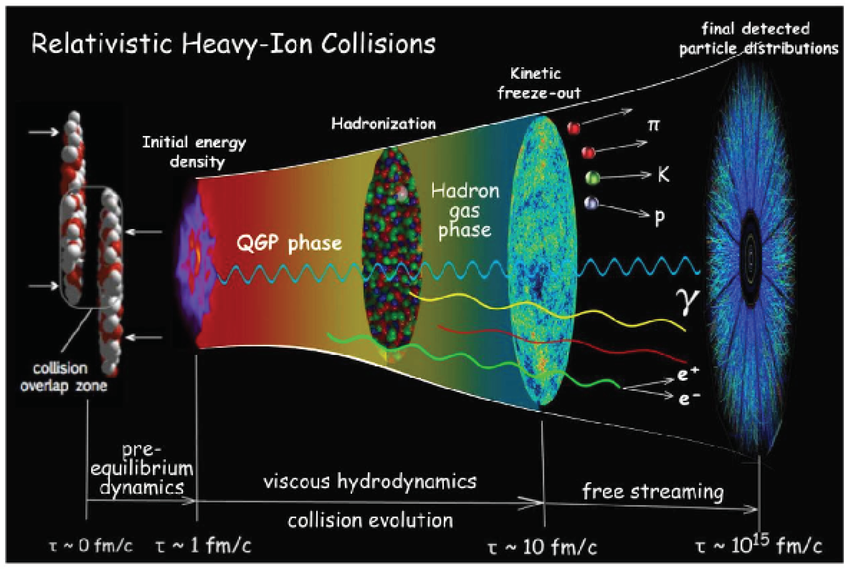
\includegraphics[width=\linewidth]{img/qgp.png}

\vspace{0.1cm}
{\tiny Schematic evolution of a relativistic heavy-ion collision.}

\end{columns}
\end{frame}

